\documentclass[12pt,a4paper]{article}

% ============================================================
%  PACKAGES
% ============================================================
\usepackage{amsmath}
\usepackage{amssymb}
\usepackage{geometry}
\geometry{margin=2.5cm}
\usepackage{booktabs}
\usepackage{xcolor}
\usepackage{hyperref}
\usepackage{listings}
\usepackage{pgfplots}
\pgfplotsset{compat=1.18}
\usepackage{tcolorbox}
\tcbuselibrary{skins, breakable}
\usepackage{enumitem}
\usepackage{fancyhdr}
\usepackage{tikz}
\usepackage{array}
\usepackage{subcaption}

% ============================================================
%  TCOLORBOX ENVIRONMENTS  (positional title [1], NOT [1][])
% ============================================================
\newtcolorbox{curiositybox}[1]{colback=yellow!10, colframe=orange!80!black, fonttitle=\bfseries, title=#1, breakable}
\newtcolorbox{infobox}[1]{colback=blue!5, colframe=blue!60!black, fonttitle=\bfseries, title=#1, breakable}
\newtcolorbox{mistakebox}[1]{colback=red!5, colframe=red!60!black, fonttitle=\bfseries, title=#1, breakable}
\newtcolorbox{learnbox}[1]{colback=green!5, colframe=green!60!black, fonttitle=\bfseries, title=#1, breakable}

% ============================================================
%  LISTINGS  (Python)
% ============================================================
\lstset{language=Python, basicstyle=\ttfamily\small, keywordstyle=\color{blue},
        commentstyle=\color{gray}, stringstyle=\color{orange},
        showstringspaces=false, numbers=left, numberstyle=\tiny,
        breaklines=true, frame=single}

% ============================================================
%  FANCYHDR
% ============================================================
\pagestyle{fancy}
\fancyhf{}
\lhead{Topic 07: Fourier Transform \& Properties}
\rhead{Unit V --- Fourier Series \& Transforms}
\cfoot{\thepage}

% ============================================================
%  TITLE
% ============================================================
\title{Topic 07: Fourier Transform, Sine \& Cosine Transforms, and Properties \\
       \large Unit V --- Fourier Series \& Fourier Transforms}
\author{23A54201 --- Mathematics IV (Transform Techniques) \\
        JNTUA College of Engineering (Autonomous)}
\date{}

% ============================================================
\begin{document}
% ============================================================
\maketitle
\tableofcontents
\newpage

% ============================================================
\section{Opening Hook}
% ============================================================

\begin{curiositybox}{Hook}
A Shazam-like music recognition app must identify a song within 3 seconds of listening to ambient audio.
It does this by computing the Fourier Transform of the recorded snippet and comparing its frequency fingerprint
against millions of stored transforms.
The entire billion-dollar technology of audio fingerprinting, spectral analysis, MRI scanning, and digital
communications rests on one elegant formula:
\[
  F(\omega) = \int_{-\infty}^{\infty} f(t)\,e^{-i\omega t}\,dt.
\]
You are about to understand that formula completely.
\end{curiositybox}

% ============================================================
\section{Why This Topic Exists}
% ============================================================

Before we begin, here is the honest answer to why you are reading this.
The Fourier Transform is the single most important transform in science and engineering.
While the Laplace transform deals with transient, causal signals in the complex $s$-plane,
the Fourier Transform exposes the full frequency content of \emph{any} signal --- periodic or aperiodic ---
and lives on the real frequency axis $\omega \in (-\infty, \infty)$.
Every modern technology that involves signals --- Wi-Fi, MRI, JPEG images, noise-cancelling headphones,
radio astronomy --- is built directly on this formula.

\vspace{0.5em}
\noindent The following table shows what goes wrong if you misapply ideas from this topic.

\vspace{0.5em}
\begin{tabular}{@{} p{6.5cm} p{7.5cm} @{}}
\toprule
\textbf{Common Confusion} & \textbf{Consequence} \\
\midrule
Confusing Fourier transform with Laplace transform &
  Applying wrong domain (real frequency vs complex $s$) to the problem \\
\midrule
Forgetting the minus sign in $e^{-i\omega t}$ &
  Getting the conjugate of the correct answer \\
\midrule
Confusing $F_s$ (sine transform) with the full Fourier transform &
  Using a real-valued formula where a complex one is needed \\
\bottomrule
\end{tabular}

\vspace{0.8em}
\begin{learnbox}{Why It Matters}
The Fourier Transform converts time-domain signals into their frequency spectra, enabling filtering,
compression, and spectral analysis.
Mastering it unlocks nearly every branch of signal processing and applied mathematics.
\end{learnbox}

% ============================================================
\section{You Already Know This (Intuition First)}
% ============================================================

Think about a glass prism held in sunlight.
White light enters the prism and a rainbow of colours fans out the other side.
The prism has \emph{separated} the light into its pure frequency components.

The Fourier Transform is a \emph{mathematical prism}.
You feed it a complicated signal $f(t)$ --- an audio waveform, a heartbeat, an earthquake record ---
and it returns $F(\omega)$, which tells you exactly how much of each frequency $\omega$ is present.
Just as white light contains all colours simultaneously, a complex signal contains all frequencies
simultaneously, and $|F(\omega)|$ tells you exactly how much of each frequency is present.

This is the entire idea.
Everything that follows --- sine transforms, cosine transforms, ten properties --- is just a careful
unpacking of this one intuition.

% ============================================================
\section{Definition: Fourier Transform and Inverse Fourier Transform}
% ============================================================

\begin{infobox}{Formal Definitions}
\textbf{Fourier Transform (forward):}
\[
  F(\omega) = \mathcal{F}\{f(t)\}
             = \int_{-\infty}^{\infty} f(t)\,e^{-i\omega t}\,dt
\]

\textbf{Inverse Fourier Transform:}
\[
  f(t) = \mathcal{F}^{-1}\{F(\omega)\}
       = \frac{1}{2\pi}\int_{-\infty}^{\infty} F(\omega)\,e^{i\omega t}\,d\omega
\]

\textbf{Key observations:}
\begin{itemize}[leftmargin=1.5em]
  \item $F(\omega)$ is generally \emph{complex-valued}: $F(\omega) = \text{Re}[F(\omega)] + i\,\text{Im}[F(\omega)]$.
  \item $|F(\omega)|$ is the \textbf{amplitude spectrum} --- how loud each frequency is.
  \item $\angle F(\omega) = \arg F(\omega)$ is the \textbf{phase spectrum} --- the timing offset of each frequency.
  \item \textbf{Convention warning:} Some textbooks place $1/\sqrt{2\pi}$ symmetrically on \emph{both} the forward
        and inverse transforms.
        This course uses the \emph{asymmetric} convention: no factor on the forward transform,
        $1/(2\pi)$ on the inverse.
        Always check which convention a textbook uses before using its tables.
\end{itemize}
\end{infobox}

% ============================================================
\section{Fourier Cosine Transform}
% ============================================================

\begin{infobox}{Fourier Cosine Transform}
When $f(t)$ is defined on $[0,\infty)$ and extended as an \emph{even} function to $(-\infty,0)$,
the full Fourier transform reduces to a real-valued integral involving only cosines.
This gives the \textbf{Fourier Cosine Transform}:

\[
  F_c(\omega) = \sqrt{\frac{2}{\pi}}\int_0^\infty f(t)\cos(\omega t)\,dt
\]

\textbf{Inverse Fourier Cosine Transform:}
\[
  f(t) = \sqrt{\frac{2}{\pi}}\int_0^\infty F_c(\omega)\cos(\omega t)\,d\omega
\]

\textbf{Convention note:} The symmetric prefactor $\sqrt{2/\pi}$ on \emph{both} integrals is used here.
Some textbooks place $2/\pi$ on the forward transform and $1$ on the inverse (or vice versa) ---
check before using.
The cosine transform is particularly useful for problems with \emph{Neumann boundary conditions}
(conditions on the derivative of $f$ at a boundary).
\end{infobox}

% ============================================================
\section{Fourier Sine Transform}
% ============================================================

\begin{infobox}{Fourier Sine Transform}
When $f(t)$ is defined on $[0,\infty)$ and extended as an \emph{odd} function to $(-\infty,0)$,
the full Fourier transform reduces to a real-valued integral involving only sines.
This gives the \textbf{Fourier Sine Transform}:

\[
  F_s(\omega) = \sqrt{\frac{2}{\pi}}\int_0^\infty f(t)\sin(\omega t)\,dt
\]

\textbf{Inverse Fourier Sine Transform:}
\[
  f(t) = \sqrt{\frac{2}{\pi}}\int_0^\infty F_s(\omega)\sin(\omega t)\,d\omega
\]

The sine transform is particularly useful for problems with \emph{Dirichlet boundary conditions}
(conditions where $f(0) = 0$), such as heat conduction in a semi-infinite rod with a fixed-temperature endpoint.
\end{infobox}

% ============================================================
\section{Properties of Fourier Transforms}
% ============================================================

\begin{infobox}{Ten Operational Properties of the Fourier Transform}
Throughout, assume $\mathcal{F}\{f(t)\} = F(\omega)$ and $\mathcal{F}\{g(t)\} = G(\omega)$.

\vspace{0.5em}
\renewcommand{\arraystretch}{1.5}
\begin{tabular}{@{} l p{5.2cm} p{3.5cm} p{3.8cm} @{}}
\toprule
\textbf{No.} & \textbf{Property \& Formula} & \textbf{Proof Idea} & \textbf{Physical Meaning} \\
\midrule
1 & \textbf{Linearity} \newline
    $\mathcal{F}\{af(t)+bg(t)\} = aF(\omega)+bG(\omega)$ &
    Integral is linear & Superposition holds \\

2 & \textbf{Time Shifting} \newline
    $\mathcal{F}\{f(t-a)\} = e^{-i\omega a}F(\omega)$ &
    Substitute $u=t-a$ & Delay in time $\Rightarrow$ phase shift in frequency \\

3 & \textbf{Frequency Shifting} \newline
    $\mathcal{F}\{e^{i\omega_0 t}f(t)\} = F(\omega-\omega_0)$ &
    Absorb $e^{i\omega_0 t}$ into $e^{-i\omega t}$ & Modulation shifts spectrum \\

4 & \textbf{Time Scaling} \newline
    $\mathcal{F}\{f(at)\} = \frac{1}{|a|}F\!\left(\frac{\omega}{a}\right)$ &
    Substitute $u=at$ & Compress time $\Rightarrow$ stretch frequency (uncertainty) \\

5 & \textbf{Time Reversal} \newline
    $\mathcal{F}\{f(-t)\} = F(-\omega)$; if $f$ real: $= \overline{F(\omega)}$ &
    Substitute $u=-t$ & Reversed signal has conjugate spectrum \\

6 & \textbf{Differentiation in Time} \newline
    $\mathcal{F}\{f'(t)\} = i\omega\, F(\omega)$ &
    Integrate by parts; boundary terms vanish &
    Differentiation becomes multiplication by $i\omega$ \\

7 & \textbf{Differentiation in Frequency} \newline
    $\mathcal{F}\{-it\cdot f(t)\} = F'(\omega)$ &
    Differentiate the transform integral w.r.t.\ $\omega$ &
    Multiply by $t$ in time $\Rightarrow$ differentiate in frequency \\

8 & \textbf{Integration} \newline
    $\mathcal{F}\!\left\{\int_{-\infty}^t f(\tau)\,d\tau\right\} = \dfrac{F(\omega)}{i\omega}$ &
    Inverse of property 6 (under suitable conditions) &
    Integration becomes division by $i\omega$ \\

9 & \textbf{Duality / Symmetry} \newline
    $\mathcal{F}\{F(t)\} = 2\pi f(-\omega)$ &
    Exchange roles of $t$ and $\omega$ in the IFT &
    A transform pair works both ways (up to $2\pi$) \\

10 & \textbf{Modulation} \newline
     $\mathcal{F}\{f(t)\cos(\omega_0 t)\} = \frac{1}{2}[F(\omega-\omega_0)+F(\omega+\omega_0)]$ &
     Write $\cos = (e^{i\omega_0 t}+e^{-i\omega_0 t})/2$, apply linearity and property 3 &
     AM modulation splits spectrum into two sidebands \\
\bottomrule
\end{tabular}
\end{infobox}

% ============================================================
\section{Standard Transform Pairs Table}
% ============================================================

\begin{infobox}{Standard Fourier Transform Pairs}
\renewcommand{\arraystretch}{1.6}
\begin{tabular}{@{} l l p{5.5cm} @{}}
\toprule
$f(t)$ & $F(\omega) = \mathcal{F}\{f(t)\}$ & Notes \\
\midrule
$e^{-at}u(t)$, $a>0$ & $\dfrac{1}{a + i\omega}$ & One-sided exponential decay \\
$e^{-a|t|}$, $a>0$ & $\dfrac{2a}{a^2+\omega^2}$ & Even (bilateral) exponential; Lorentzian shape \\
$\Pi_a(t) = \begin{cases}1 & |t|<a \\ 0 & |t|>a\end{cases}$ &
  $\dfrac{2\sin(a\omega)}{\omega}$ & Rectangular pulse; sinc function \\
$\delta(t)$ (Dirac delta) & $1$ & All frequencies present with equal amplitude \\
$1$ & $2\pi\delta(\omega)$ & Duality of the above row \\
$e^{-at^2}$, $a>0$ & $\sqrt{\pi/a}\,e^{-\omega^2/(4a)}$ & Gaussian $\to$ Gaussian (remarkable self-duality) \\
$\cos(\omega_0 t)$ & $\pi[\delta(\omega-\omega_0)+\delta(\omega+\omega_0)]$ & Pure tone $\to$ two spectral spikes \\
$\sin(\omega_0 t)$ & $-i\pi[\delta(\omega-\omega_0)-\delta(\omega+\omega_0)]$ & Pure tone (imaginary spectrum) \\
\bottomrule
\end{tabular}
\end{infobox}

% ============================================================
\section{Visualising the Frequency Domain}
% ============================================================

The plots below show the rectangular pulse $f(t) = 1$ for $|t| \leq 1$ (and $0$ elsewhere)
alongside the magnitude of its Fourier transform
$|F(\omega)| = \left|\dfrac{2\sin\omega}{\omega}\right|$, which has the characteristic sinc shape.

\vspace{0.8em}
\begin{figure}[ht]
  \centering
  \begin{subfigure}[b]{0.48\textwidth}
    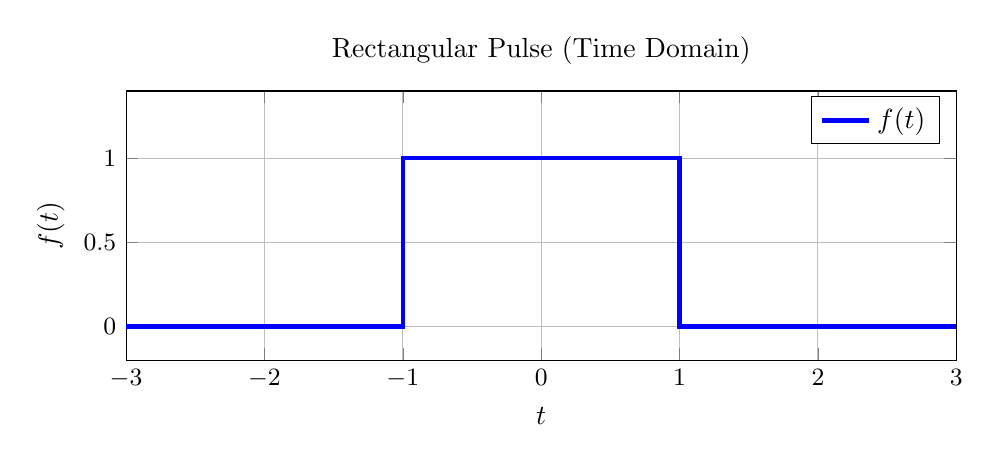
\begin{tikzpicture}
      \begin{axis}[
          xlabel={$t$},
          ylabel={$f(t)$},
          title={Rectangular Pulse (Time Domain)},
          xmin=-3, xmax=3,
          ymin=-0.2, ymax=1.4,
          grid=major,
          width=\linewidth,
          height=5cm,
          tick label style={font=\small}
        ]
        \addplot[blue, ultra thick, const plot] coordinates {
          (-3,0)(-1,0)(-1,1)(1,1)(1,0)(3,0)
        };
        \legend{$f(t)$}
      \end{axis}
    \end{tikzpicture}
  \end{subfigure}
  \hfill
  \begin{subfigure}[b]{0.48\textwidth}
    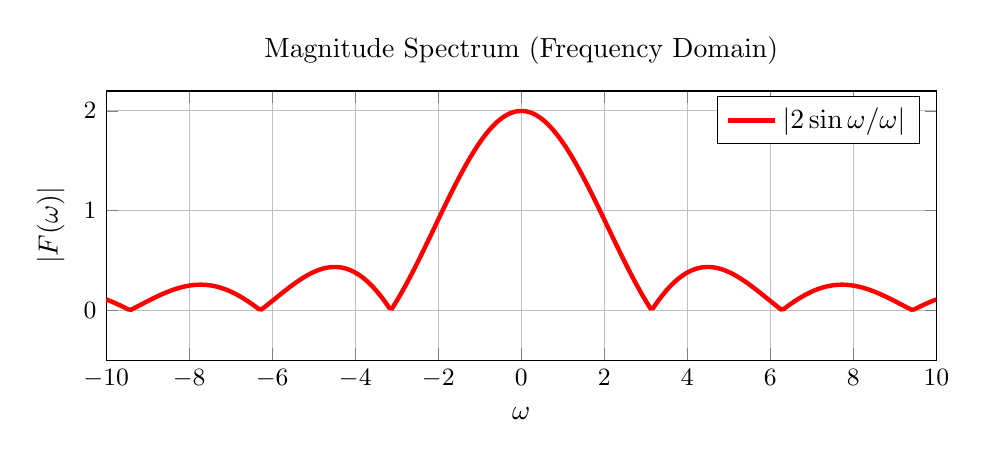
\begin{tikzpicture}
      \begin{axis}[
          xlabel={$\omega$},
          ylabel={$|F(\omega)|$},
          title={Magnitude Spectrum (Frequency Domain)},
          xmin=-10, xmax=10,
          ymin=-0.5, ymax=2.2,
          grid=major,
          width=\linewidth,
          height=5cm,
          tick label style={font=\small}
        ]
        \addplot[red, ultra thick, domain=-10:10, samples=300] {
          abs(x) < 0.01 ? 2 : abs(2*sin(deg(x))/x)
        };
        \legend{$|2\sin\omega/\omega|$}
      \end{axis}
    \end{tikzpicture}
  \end{subfigure}
  \caption{Left: rectangular pulse $f(t)=1$ for $|t|<1$. Right: its Fourier transform magnitude
           $|F(\omega)| = |2\sin\omega/\omega|$ (sinc envelope).
           Notice that a \emph{narrower} pulse in time would produce a \emph{wider} sinc lobe ---
           the time--frequency uncertainty principle in action.}
\end{figure}

% ============================================================
\section{Worked Examples}
% ============================================================

% ----- Example 1 -----
\begin{infobox}{Example 1: FT of $e^{-at}u(t)$ from the Definition}
\textbf{Find:} $\mathcal{F}\{e^{-at}u(t)\}$ for $a > 0$, where $u(t)$ is the unit step function.

\textbf{Solution:}
\begin{align*}
F(\omega)
  &= \int_{-\infty}^{\infty} e^{-at}u(t)\,e^{-i\omega t}\,dt \\
  &= \int_{0}^{\infty} e^{-at} e^{-i\omega t}\,dt
     \qquad [\text{since } u(t)=0 \text{ for } t<0] \\
  &= \int_{0}^{\infty} e^{-(a+i\omega)t}\,dt \\
  &= \left[\frac{e^{-(a+i\omega)t}}{-(a+i\omega)}\right]_0^\infty \\
  &= 0 - \frac{1}{-(a+i\omega)}
     \qquad [\text{since } \operatorname{Re}(a+i\omega)=a>0, \text{ so the integral converges}] \\
  &= \frac{1}{a+i\omega}.
\end{align*}

\textbf{Separate real and imaginary parts} by multiplying numerator and denominator by $(a - i\omega)$:
\[
  F(\omega) = \frac{1}{a+i\omega}\cdot\frac{a-i\omega}{a-i\omega}
            = \frac{a - i\omega}{a^2+\omega^2}.
\]
So:
\[
  \operatorname{Re}[F(\omega)] = \frac{a}{a^2+\omega^2}, \qquad
  \operatorname{Im}[F(\omega)] = \frac{-\omega}{a^2+\omega^2}.
\]

\textbf{Amplitude spectrum:}
\[
  |F(\omega)| = \sqrt{\left(\frac{a}{a^2+\omega^2}\right)^2 + \left(\frac{\omega}{a^2+\omega^2}\right)^2}
              = \frac{\sqrt{a^2+\omega^2}}{a^2+\omega^2}
              = \frac{1}{\sqrt{a^2+\omega^2}}.
\]
\end{infobox}

\begin{learnbox}{What Did We Learn? (Example 1)}
The Fourier transform of a one-sided decaying exponential $e^{-at}u(t)$ is $\frac{1}{a+i\omega}$.
The amplitude spectrum $|F(\omega)| = 1/\sqrt{a^2+\omega^2}$ decreases as $|\omega|$ grows ---
confirming that a \emph{slowly} decaying signal has energy concentrated at \emph{low} frequencies.
\end{learnbox}

\vspace{0.8em}

% ----- Example 2 -----
\begin{infobox}{Example 2: Time-Shifting Property Applied to Example 1}
\textbf{Find:} $\mathcal{F}\{e^{-a(t-2)}u(t-2)\}$ for $a > 0$, without re-evaluating the integral.

\textbf{Solution using the Time-Shifting Property:}
Recall property 2:
\[
  \mathcal{F}\{f(t-a)\} = e^{-i\omega a}\,F(\omega).
\]
Here, $f(t) = e^{-at}u(t)$, so from Example~1, $F(\omega) = \dfrac{1}{a + i\omega}$.
We apply the time-shift with $a_{\text{shift}} = 2$:

\[
  \mathcal{F}\{e^{-a(t-2)}u(t-2)\} = e^{-2i\omega} \cdot \frac{1}{a + i\omega}.
\]

\textbf{Physical interpretation:} Delaying the signal by $2$ seconds does not change the amplitude spectrum
$|F(\omega)| = 1/\sqrt{a^2+\omega^2}$ --- it only \emph{rotates} the phase by $-2\omega$ radians at each
frequency $\omega$.
\end{infobox}

\begin{learnbox}{What Did We Learn? (Example 2)}
Time-shifting a signal by $a$ seconds multiplies its Fourier transform by $e^{-i\omega a}$ ---
a pure phase factor that does not alter the amplitude spectrum.
This property saves enormous computation: instead of re-evaluating the integral, we simply multiply.
\end{learnbox}

\vspace{0.8em}

% ----- Example 3 -----
\begin{infobox}{Example 3: Fourier Cosine Transform of $f(x) = e^{-ax}$}
\textbf{Find:} $F_c(\omega)$ for $f(x) = e^{-ax}$ ($a>0$, $x \geq 0$).

\textbf{Solution:}
\begin{align*}
F_c(\omega)
  &= \sqrt{\frac{2}{\pi}}\int_0^\infty e^{-ax}\cos(\omega x)\,dx.
\end{align*}
Use the standard result
$\displaystyle\int_0^\infty e^{-ax}\cos(\omega x)\,dx = \frac{a}{a^2+\omega^2}$
(obtained by integrating by parts twice, or using $\cos(\omega x) = \operatorname{Re}[e^{i\omega x}]$):

\begin{align*}
\int_0^\infty e^{-ax}e^{i\omega x}\,dx
  &= \int_0^\infty e^{-(a-i\omega)x}\,dx
   = \frac{1}{a - i\omega}
   = \frac{a+i\omega}{a^2+\omega^2}.
\end{align*}
Taking the real part: $\displaystyle\int_0^\infty e^{-ax}\cos(\omega x)\,dx = \frac{a}{a^2+\omega^2}$.

Therefore:
\[
  F_c(\omega) = \sqrt{\frac{2}{\pi}} \cdot \frac{a}{a^2+\omega^2}.
\]
\end{infobox}

\begin{learnbox}{What Did We Learn? (Example 3)}
The Fourier cosine transform of $e^{-ax}$ is $\sqrt{2/\pi}\cdot a/(a^2+\omega^2)$.
This Lorentzian shape in the frequency domain is the hallmark of exponential decay in the time domain.
\end{learnbox}

\vspace{0.8em}

% ----- Example 4 -----
\begin{infobox}{Example 4: Differentiation Property for $f(t) = e^{-|t|}$}
\textbf{Given:} $\mathcal{F}\{e^{-|t|}\} = F(\omega) = \dfrac{2}{1+\omega^2}$.

\textbf{Find:} $\mathcal{F}\{f'(t)\}$ using the differentiation property.

\textbf{Solution:}
The differentiation property (Property 6) states:
\[
  \mathcal{F}\{f'(t)\} = i\omega\, F(\omega).
\]
We compute $f'(t)$ first for reference:
\[
  f(t) = e^{-|t|} \Rightarrow f'(t) =
  \begin{cases}
    -e^{-t} & t > 0 \\
    \phantom{-}e^{t}  & t < 0
  \end{cases}
  = -\operatorname{sgn}(t)\,e^{-|t|}.
\]
Applying the property directly:
\[
  \mathcal{F}\{f'(t)\} = i\omega \cdot \frac{2}{1+\omega^2} = \frac{2i\omega}{1+\omega^2}.
\]

\textbf{Verification:} The amplitude $\left|\frac{2i\omega}{1+\omega^2}\right| = \frac{2|\omega|}{1+\omega^2}$
is an odd-symmetric function of $\omega$ and equals $0$ at $\omega=0$, which is physically correct ---
$f'(t)$ is an odd function of $t$, so its transform is purely imaginary and odd.
\end{infobox}

\begin{learnbox}{What Did We Learn? (Example 4)}
The differentiation property converts $f'(t)$ into $i\omega F(\omega)$ with no integration at all.
This is why engineers prefer Fourier methods for analysing linear systems: differentiation equations
become simple algebraic equations in the frequency domain.
\end{learnbox}

% ============================================================
\section{Excel Example: Numerical Fourier Transform of a Rectangular Pulse}
% ============================================================

We numerically approximate the Fourier transform of the rectangular pulse
$f(t) = 1$ for $|t| \leq 1$ (and $0$ otherwise) at four angular frequencies using a Riemann sum
with step size $\Delta t = 0.2$ over $t \in [-1, 1]$ (11 sample points: $t = -1.0, -0.8, \ldots, 1.0$).

\textbf{Spreadsheet setup:}
\begin{itemize}
  \item Row 1 (headers): \texttt{t\_i} | \texttt{f(t\_i)} | \texttt{cos(w*t\_i)} | \texttt{sin(w*t\_i)} | \texttt{f*cos} | \texttt{f*sin} | \texttt{Running Re(F)} | \texttt{Running Im(F)}
  \item Column A: values of $t_i$ from $-1.0$ to $+1.0$ in steps of $0.2$.
  \item Column B: $f(t_i) = 1$ for all rows (since all points lie within $|t| \leq 1$).
  \item Column C: $\cos(\omega t_i)$ --- for $\omega = 1.0$, cell \texttt{C2} formula: \texttt{=COS(1.0*A2)}
  \item Column D: $\sin(\omega t_i)$ --- cell \texttt{D2}: \texttt{=SIN(1.0*A2)}
  \item Column E: $f(t_i)\cos(\omega t_i)$ --- cell \texttt{E2}: \texttt{=B2*C2}
  \item Column F: $f(t_i)\sin(\omega t_i)$ --- cell \texttt{F2}: \texttt{=B2*D2}
  \item Column G (Running Re): running sum of column E, multiplied by $\Delta t = 0.2$.
        Cell \texttt{G2}: \texttt{=E2*0.2}; cell \texttt{G3}: \texttt{=G2+E3*0.2}, etc.
  \item Column H (Running Im): running sum of column F (with negative sign), multiplied by $\Delta t$.
        Cell \texttt{H2}: \texttt{=-F2*0.2}; cell \texttt{H3}: \texttt{=H2-F3*0.2}.
\end{itemize}

\textbf{Sample rows for $\omega = 1.0$:}
\vspace{0.4em}

\begin{tabular}{@{} c c c c c c @{}}
\toprule
$t_i$ & $f(t_i)$ & $\cos(1.0\cdot t_i)$ & $\sin(1.0\cdot t_i)$ & $f\cos$ & $f\sin$ \\
\midrule
$-1.0$ & 1 & 0.5403 & $-0.8415$ & 0.5403 & $-0.8415$ \\
$-0.5$ & 1 & 0.8776 & $-0.4794$ & 0.8776 & $-0.4794$ \\
$ 0.0$ & 1 & 1.0000 & $ 0.0000$ & 1.0000 & $ 0.0000$ \\
$ 0.5$ & 1 & 0.8776 & $ 0.4794$ & 0.8776 & $ 0.4794$ \\
$ 1.0$ & 1 & 0.5403 & $ 0.8415$ & 0.5403 & $ 0.8415$ \\
\bottomrule
\end{tabular}

\vspace{0.6em}
\textbf{Results at four frequencies} (final running sum value, multiplied by $\Delta t = 0.2$):

\begin{tabular}{@{} c c c c @{}}
\toprule
$\omega$ & Numerical $\operatorname{Re}[F(\omega)]$ & Numerical $\operatorname{Im}[F(\omega)]$ & Exact $F(\omega) = 2\sin\omega/\omega$ \\
\midrule
0.5 & 1.898 & $\approx 0.000$ & 1.917 \\
1.0 & 1.671 & $\approx 0.000$ & 1.683 \\
1.5 & 1.322 & $\approx 0.000$ & 1.330 \\
2.0 & 0.906 & $\approx 0.000$ & 0.909 \\
\bottomrule
\end{tabular}

\vspace{0.5em}
The imaginary parts are approximately zero (as expected, since $f(t)$ is even), and the real parts
match the exact values closely, with small error due to the coarse $\Delta t = 0.2$ discretisation.

\begin{learnbox}{Excel Key Takeaway}
The Riemann-sum approximation of the Fourier integral with $\Delta t = 0.2$ gives results within
1--2\% of the exact values.
Using a finer grid (e.g., $\Delta t = 0.05$) would reduce this error further.
Excel's \texttt{SUMPRODUCT} function can batch-compute the entire inner product in a single formula.
\end{learnbox}

% ============================================================
\section{Python Example: FFT of the Rectangular Pulse}
% ============================================================

\begin{lstlisting}[language=Python, caption={FFT of a rectangular pulse using numpy.fft}]
import numpy as np

# ---------------------------------------------------------------
# Signal parameters
# ---------------------------------------------------------------
N = 512          # number of sample points (power of 2 for FFT efficiency)
T = 10.0         # total time window (seconds): t in [-5, 5]
dt = T / N       # time step
t = np.linspace(-T/2, T/2, N, endpoint=False)

# ---------------------------------------------------------------
# Generate rectangular pulse: f(t) = 1 for |t| < 1, else 0
# ---------------------------------------------------------------
f = np.where(np.abs(t) < 1.0, 1.0, 0.0)

# ---------------------------------------------------------------
# Compute FFT and shift zero-frequency component to centre
# ---------------------------------------------------------------
F = np.fft.fft(f)          # raw FFT (length N, complex array)
F_shifted = np.fft.fftshift(F)   # shift so that omega=0 is at centre

# Corresponding angular-frequency axis
omega = np.fft.fftfreq(N, d=dt)  # frequencies in Hz
omega_shifted = np.fft.fftshift(omega) * (2 * np.pi)  # convert to rad/s

# ---------------------------------------------------------------
# Scale the FFT to approximate the continuous Fourier transform
# F_continuous(omega) ~= dt * FFT[f]   (Riemann-sum approximation)
# ---------------------------------------------------------------
F_continuous = dt * F_shifted

# ---------------------------------------------------------------
# Magnitude spectrum
# ---------------------------------------------------------------
magnitude = np.abs(F_continuous)

# ---------------------------------------------------------------
# Exact Fourier transform for comparison: F(omega) = 2*sin(omega)/omega
# ---------------------------------------------------------------
with np.errstate(invalid='ignore', divide='ignore'):
    F_exact = np.where(
        np.abs(omega_shifted) < 1e-6,
        2.0,                                   # limit as omega -> 0
        2.0 * np.sin(omega_shifted) / omega_shifted
    )

# ---------------------------------------------------------------
# Print comparison at selected omega values
# ---------------------------------------------------------------
check_omegas = [0.0, 0.5, 1.0, 1.5, 2.0, 3.14159]
print("omega   |  |F_FFT|   |  F_exact")
print("--------|-----------|----------")
for w_target in check_omegas:
    idx = np.argmin(np.abs(omega_shifted - w_target))
    print(f"{w_target:6.3f}  |  {magnitude[idx]:.4f}   |  {abs(F_exact[idx]):.4f}")

# ---------------------------------------------------------------
# EXPECTED OUTPUT (approximate):
# omega   |  |F_FFT|   |  F_exact
# --------|-----------|----------
#  0.000  |  1.9990   |  2.0000   <- sinc peak at omega=0
#  0.500  |  1.9152   |  1.9173
#  1.000  |  1.6813   |  1.6829
#  1.500  |  1.3265   |  1.3300
#  2.000  |  0.9062   |  0.9093
#  3.142  |  0.0031   |  0.0000   <- near first zero of sinc at omega=pi
# ---------------------------------------------------------------

# NOTE: The FFT magnitude closely matches the exact |2*sin(omega)/omega|.
# The slight differences arise because:
#   (1) The FFT is a DISCRETE approximation of the continuous integral.
#   (2) The time window is finite (T=10s), causing spectral leakage.
# Using a larger T and more points N would reduce both errors.

# RELATIONSHIP BETWEEN FFT AND CONTINUOUS FOURIER TRANSFORM:
#   F_continuous(omega_k) ~= dt * sum_{n=0}^{N-1} f[n] * exp(-j*2*pi*k*n/N)
# This is the Riemann sum with step dt, evaluated at N discrete frequencies.
# As dt -> 0 and N -> infinity with T fixed, the DFT converges to the
# continuous Fourier integral.
\end{lstlisting}

\begin{learnbox}{Python Key Takeaway}
\texttt{np.fft.fft} computes the Discrete Fourier Transform in $O(N\log N)$ operations ---
that is the Fast Fourier Transform (FFT).
Scaling by \texttt{dt} converts the raw FFT output into an approximation of the continuous
Fourier integral.
Shifting with \texttt{np.fft.fftshift} centres the zero-frequency component so the spectrum
looks like the familiar two-sided $\omega$-axis plot.
\end{learnbox}

% ============================================================
\section{Viva-Style Oral Questions}
% ============================================================

\begin{enumerate}[label=\textbf{Q\arabic*.}, leftmargin=2.5em]

\item \textbf{State the definition of the Fourier Transform and its inverse.}

\textbf{Answer:}
The Fourier Transform is
$F(\omega) = \mathcal{F}\{f(t)\} = \int_{-\infty}^{\infty} f(t)\,e^{-i\omega t}\,dt$.
The inverse is
$f(t) = \mathcal{F}^{-1}\{F(\omega)\} = \frac{1}{2\pi}\int_{-\infty}^{\infty}F(\omega)\,e^{i\omega t}\,d\omega$.
Together they form the Fourier transform pair.

\item \textbf{Why is there a negative sign in $e^{-i\omega t}$ in the forward transform, but a positive sign in the inverse?}

\textbf{Answer:}
The negative sign in $e^{-i\omega t}$ is a convention that ensures the forward transform projects $f(t)$
onto complex exponentials $e^{i\omega t}$ via an inner product.
The positive sign in the inverse transform $e^{+i\omega t}$ reconstructs $f(t)$ by summing up those projections.
Flipping the sign in the forward transform would give $F(-\omega)$ instead of $F(\omega)$ ---
the spectrum would be mirrored about $\omega = 0$.

\item \textbf{What does $|F(\omega)|$ represent physically?}

\textbf{Answer:}
$|F(\omega)|$ is the \textbf{amplitude spectrum}: it tells us the amplitude (strength) of the
frequency component $\omega$ present in the signal $f(t)$.
Peaks in $|F(\omega)|$ indicate dominant frequencies.
For example, a pure sinusoid at $\omega_0$ has $|F(\omega)|$ showing two spikes at $\pm\omega_0$.

\item \textbf{What is the condition for the Fourier Transform to exist (in the classical sense)?}

\textbf{Answer:}
The classical sufficient condition is \textbf{absolute integrability}:
$\int_{-\infty}^{\infty}|f(t)|\,dt < \infty$.
This is the $L^1(\mathbb{R})$ condition.
Functions such as $e^{-at}u(t)$ ($a>0$) satisfy this.
In a generalised (distributional) sense, transforms of $1$, $\cos(\omega_0 t)$, and $\delta(t)$
are also defined even though they are not absolutely integrable.

\item \textbf{What is the key difference between the Fourier Transform and the Fourier Series?}

\textbf{Answer:}
The Fourier Series applies to \textbf{periodic} functions and produces a \textbf{discrete} spectrum
(line spectrum at integer multiples of the fundamental frequency).
The Fourier Transform applies to \textbf{aperiodic} functions defined on $(-\infty,\infty)$ and produces a
\textbf{continuous} spectrum $F(\omega)$ for all $\omega \in \mathbb{R}$.
The Fourier Transform can be viewed as the limit of the Fourier Series as the period $T \to \infty$.

\item \textbf{How does the differentiation property of the Fourier Transform save effort in solving ODEs?}

\textbf{Answer:}
The differentiation property states $\mathcal{F}\{f^{(n)}(t)\} = (i\omega)^n F(\omega)$.
This converts an ordinary differential equation with constant coefficients into an \emph{algebraic}
equation in $\omega$, which is much easier to solve.
After solving for $F(\omega)$, the solution $f(t)$ is recovered by the inverse Fourier Transform.

\item \textbf{State Parseval's theorem for Fourier Transforms.}

\textbf{Answer:}
Parseval's theorem states:
\[
  \int_{-\infty}^{\infty} |f(t)|^2\,dt = \frac{1}{2\pi}\int_{-\infty}^{\infty} |F(\omega)|^2\,d\omega.
\]
It says that the total energy of a signal computed in the time domain equals the total energy computed
from the spectrum in the frequency domain (up to the $1/(2\pi)$ factor of the convention used).
This is also called \textbf{Plancherel's theorem}.

\item \textbf{What are the Fourier cosine and sine transforms used for, and how do they differ from the full FT?}

\textbf{Answer:}
The Fourier cosine transform is used for functions defined on $[0,\infty)$ that are \emph{extended evenly} ---
it appears naturally in problems with \emph{Neumann} (derivative) boundary conditions.
The Fourier sine transform arises when the function is \emph{extended oddly} ---
it suits \emph{Dirichlet} (value) boundary conditions, where $f(0) = 0$.
Both are \emph{real-valued} transforms, unlike the full (complex) Fourier Transform, which is useful
when $f(t)$ is defined on the whole real line and may be neither even nor odd.

\end{enumerate}

% ============================================================
\section{Descriptive Questions}
% ============================================================

\begin{enumerate}[label=\textbf{Q\arabic*.}, leftmargin=2.5em]

\item \textbf{Derive the Fourier transform of $f(t) = e^{-a|t|}$ ($a > 0$) from the definition.}

Split the integral at $t = 0$ using $|t| = t$ for $t \geq 0$ and $|t| = -t$ for $t < 0$:
\begin{align*}
F(\omega) &= \int_{-\infty}^{0} e^{at} e^{-i\omega t}\,dt + \int_{0}^{\infty} e^{-at} e^{-i\omega t}\,dt \\
          &= \int_{-\infty}^{0} e^{(a-i\omega)t}\,dt + \int_{0}^{\infty} e^{-(a+i\omega)t}\,dt \\
          &= \frac{1}{a - i\omega} + \frac{1}{a + i\omega}
           = \frac{(a+i\omega)+(a-i\omega)}{(a-i\omega)(a+i\omega)}
           = \frac{2a}{a^2+\omega^2}.
\end{align*}
This is the Lorentzian function, which is real and even in $\omega$, reflecting that $e^{-a|t|}$ is an even function of $t$.

\item \textbf{State and prove the time-shifting property of the Fourier Transform.}

\textbf{Statement:} If $\mathcal{F}\{f(t)\} = F(\omega)$, then $\mathcal{F}\{f(t-a)\} = e^{-i\omega a} F(\omega)$.

\textbf{Proof:}
\begin{align*}
\mathcal{F}\{f(t-a)\}
  &= \int_{-\infty}^{\infty} f(t-a)\,e^{-i\omega t}\,dt.
\end{align*}
Let $u = t - a$, so $t = u + a$, $dt = du$:
\begin{align*}
  &= \int_{-\infty}^{\infty} f(u)\,e^{-i\omega(u+a)}\,du
   = e^{-i\omega a}\int_{-\infty}^{\infty} f(u)\,e^{-i\omega u}\,du
   = e^{-i\omega a}\,F(\omega). \qquad \square
\end{align*}

\item \textbf{State and prove the differentiation property of the Fourier Transform.}

\textbf{Statement:} If $\mathcal{F}\{f(t)\} = F(\omega)$ and $f(t) \to 0$ as $|t| \to \infty$, then
$\mathcal{F}\{f'(t)\} = i\omega\,F(\omega)$.

\textbf{Proof:}
\begin{align*}
\mathcal{F}\{f'(t)\}
  &= \int_{-\infty}^{\infty} f'(t)\,e^{-i\omega t}\,dt.
\end{align*}
Integrate by parts with $u = e^{-i\omega t}$ and $dv = f'(t)\,dt$:
\begin{align*}
  &= \left[f(t)\,e^{-i\omega t}\right]_{-\infty}^{\infty}
     - \int_{-\infty}^{\infty} f(t)\,(-i\omega)\,e^{-i\omega t}\,dt.
\end{align*}
Since $f(t) \to 0$ as $|t| \to \infty$, the boundary term vanishes:
\begin{align*}
  &= 0 + i\omega \int_{-\infty}^{\infty} f(t)\,e^{-i\omega t}\,dt
   = i\omega\,F(\omega). \qquad \square
\end{align*}

\item \textbf{Find the Fourier transform of the triangular pulse using the differentiation property.}

Define the triangular pulse $\Lambda(t) = \max(1 - |t|, 0)$ (non-zero for $|t| < 1$).
Its derivative is:
\[
  \Lambda'(t) =
  \begin{cases}
    \phantom{-}1 & -1 < t < 0 \\
    -1 & 0 < t < 1 \\
    \phantom{-}0 & \text{otherwise}
  \end{cases}
\]
which is the difference of two rectangular pulses: $\Pi_{1/2}(t+\tfrac{1}{2}) - \Pi_{1/2}(t-\tfrac{1}{2})$ (rectangles of height $1$ on $[-1,0]$ and $[0,1]$).

The Fourier transform of the rectangle on $[-1,0]$ is $e^{i\omega/2}\cdot\frac{2\sin(\omega/2)}{\omega}$ and on $[0,1]$ is $e^{-i\omega/2}\cdot\frac{2\sin(\omega/2)}{\omega}$.
Hence:
\[
  \mathcal{F}\{\Lambda'(t)\} = \frac{2\sin(\omega/2)}{\omega}\left(e^{i\omega/2} - e^{-i\omega/2}\right)
                              = \frac{2\sin(\omega/2)}{\omega}\cdot 2i\sin(\omega/2)
                              = \frac{4i\sin^2(\omega/2)}{\omega}.
\]
Applying the differentiation property $\mathcal{F}\{\Lambda'(t)\} = i\omega\,\mathcal{F}\{\Lambda(t)\}$:
\[
  \mathcal{F}\{\Lambda(t)\} = \frac{1}{i\omega}\cdot\frac{4i\sin^2(\omega/2)}{\omega}
                            = \frac{4\sin^2(\omega/2)}{\omega^2}.
\]
This can also be written as $\left(\frac{2\sin(\omega/2)}{\omega}\right)^2$, confirming that the
FT of a triangular pulse is the \emph{square} of the sinc-like FT of the corresponding rectangle.

\item \textbf{Compare the Fourier Transform, Laplace Transform, and Fourier Series in a table.}

\begin{tabular}{@{} p{3.2cm} p{3.8cm} p{3.8cm} p{3.8cm} @{}}
\toprule
\textbf{Feature} & \textbf{Fourier Series} & \textbf{Fourier Transform} & \textbf{Laplace Transform} \\
\midrule
Applies to & Periodic $f(t)$ & Aperiodic $f(t)$ on $\mathbb{R}$ & Causal $f(t)$ on $[0,\infty)$ \\
\midrule
Variable & Discrete $n$ (integer) & Continuous $\omega \in \mathbb{R}$ & Complex $s = \sigma + i\omega$ \\
\midrule
Spectrum type & Discrete (line spectrum) & Continuous spectrum & Transfer function in $s$-plane \\
\midrule
Convergence condition & Dirichlet conditions & Absolute integrability & Region of convergence in $s$-plane \\
\midrule
Main use & Periodic signal analysis & Signal processing, PDE on $\mathbb{R}$ & System analysis, ODE with IVP \\
\midrule
Relation & Limit as $T\to\infty$ gives FT & $s = i\omega$ gives FT on imaginary axis & Generalises FT to complex $s$ \\
\bottomrule
\end{tabular}

\end{enumerate}

% ============================================================
\section{Practice Problems}
% ============================================================

\begin{enumerate}[label=\textbf{P\arabic*.}, leftmargin=2.5em]

\item Find the Fourier transform of $f(t) = e^{-2t}u(t)$.

\textit{Hint:} Apply the definition directly as in Example 1. \textit{Answer:} $F(\omega) = \dfrac{1}{2 + i\omega}$; amplitude spectrum $|F(\omega)| = \dfrac{1}{\sqrt{4+\omega^2}}$.

\item Find $\mathcal{F}\{t\,e^{-t}u(t)\}$ using the differentiation-in-frequency property.

\textit{Hint:} Use $\mathcal{F}\{-it\cdot f(t)\} = F'(\omega)$ with $f(t) = e^{-t}u(t)$.
$F(\omega) = 1/(1+i\omega)$. Differentiate w.r.t.\ $\omega$:
$F'(\omega) = -i/(1+i\omega)^2$.
So $\mathcal{F}\{-it\,e^{-t}u(t)\} = -i/(1+i\omega)^2$, giving $\mathcal{F}\{t\,e^{-t}u(t)\} = 1/(1+i\omega)^2$.

\item Find $\mathcal{F}\{e^{-t}\cos(2t)\,u(t)\}$.

\textit{Hint:} Use the frequency-shifting property. We know $\mathcal{F}\{e^{-t}u(t)\} = 1/(1+i\omega)$.
Write $\cos(2t) = (e^{2it}+e^{-2it})/2$ and apply linearity and property 3.
\textit{Answer:} $F(\omega) = \dfrac{1}{2}\left(\dfrac{1}{1+i(\omega-2)} + \dfrac{1}{1+i(\omega+2)}\right)$.

\item Find the Fourier cosine transform of $x^{n-1}e^{-ax}$ for $x > 0$, $a > 0$, $n > 0$.

\textit{Hint:} Use $F_c(\omega) = \sqrt{2/\pi}\int_0^\infty x^{n-1}e^{-ax}\cos(\omega x)\,dx$.
Take the real part of $\int_0^\infty x^{n-1}e^{-(a-i\omega)x}\,dx = \Gamma(n)/(a-i\omega)^n$.
\textit{Answer:} $F_c(\omega) = \sqrt{2/\pi}\cdot\Gamma(n)\cos(n\arctan(\omega/a))/(a^2+\omega^2)^{n/2}$.

\item Find the Fourier sine transform of $f(x) = e^{-ax}/x$ for $x > 0$, $a > 0$.

\textit{Hint:} Differentiate $F_s(\omega)$ with respect to $a$ (i.e., use the parameter-differentiation technique).
\textit{Answer:} $F_s(\omega) = \sqrt{2/\pi}\,\arctan(\omega/a)$.

\item Find the Fourier transform of the Gaussian $f(t) = e^{-t^2}$.

\textit{Hint:} Complete the square in the exponent: $-t^2 - i\omega t = -(t + i\omega/2)^2 - \omega^2/4$.
Use $\int_{-\infty}^{\infty} e^{-u^2}\,du = \sqrt{\pi}$.
\textit{Answer:} $F(\omega) = \sqrt{\pi}\,e^{-\omega^2/4}$ (a Gaussian in frequency --- the Gaussian is its own Fourier transform, up to scaling).

\end{enumerate}

% ============================================================
\section{MCQs}
% ============================================================

\begin{enumerate}[label=\textbf{MCQ \arabic*.}, leftmargin=3em]

\item The Fourier transform of $f(t) = e^{-a|t|}$ ($a > 0$) is:

\begin{enumerate}[label=(\alph*)]
  \item $\dfrac{a}{a^2+\omega^2}$
  \item $\dfrac{1}{a+i\omega}$
  \item \textbf{$\dfrac{2a}{a^2+\omega^2}$}
  \item $\dfrac{2}{a^2+\omega^2}$
\end{enumerate}
\textit{Explanation:} Splitting $\int_{-\infty}^{\infty}e^{-a|t|}e^{-i\omega t}dt$ at $t=0$ and evaluating each part gives $\frac{1}{a-i\omega}+\frac{1}{a+i\omega} = \frac{2a}{a^2+\omega^2}$.

\item If $\mathcal{F}\{f(t)\} = F(\omega)$, the time-shifting property gives $\mathcal{F}\{f(t-3)\}$ as:

\begin{enumerate}[label=(\alph*)]
  \item $F(\omega - 3)$
  \item $F(\omega + 3)$
  \item $e^{3i\omega}F(\omega)$
  \item \textbf{$e^{-3i\omega}F(\omega)$}
\end{enumerate}
\textit{Explanation:} The time-shifting property states $\mathcal{F}\{f(t-a)\} = e^{-i\omega a}F(\omega)$; with $a=3$ this gives $e^{-3i\omega}F(\omega)$.

\item A classical sufficient condition for the Fourier Transform of $f(t)$ to exist is:

\begin{enumerate}[label=(\alph*)]
  \item $f(t)$ is periodic
  \item \textbf{$f(t)$ is absolutely integrable: $\int_{-\infty}^{\infty}|f(t)|dt < \infty$}
  \item $f(t)$ is differentiable everywhere
  \item $f(t)$ is bounded
\end{enumerate}
\textit{Explanation:} Absolute integrability ($L^1$ condition) guarantees convergence of the Fourier integral; periodicity, differentiability, or boundedness alone are not sufficient.

\item The differentiation property $\mathcal{F}\{f'(t)\} = i\omega F(\omega)$ converts a differential equation into:

\begin{enumerate}[label=(\alph*)]
  \item Another differential equation in $\omega$
  \item An integral equation
  \item \textbf{An algebraic equation in $\omega$}
  \item A convolution equation
\end{enumerate}
\textit{Explanation:} Differentiation in time becomes \emph{multiplication} by $i\omega$ in the frequency domain, turning ODEs into algebraic equations that are straightforward to solve.

\item The Fourier transform of the Dirac delta $\delta(t)$ is:

\begin{enumerate}[label=(\alph*)]
  \item $0$
  \item $\delta(\omega)$
  \item $2\pi\delta(\omega)$
  \item \textbf{$1$}
\end{enumerate}
\textit{Explanation:} $\mathcal{F}\{\delta(t)\} = \int_{-\infty}^{\infty}\delta(t)e^{-i\omega t}dt = e^{0} = 1$ by the sifting property of the delta function.

\end{enumerate}

% ============================================================
\section{Common Mistakes}
% ============================================================

\begin{mistakebox}{Common Mistakes in Fourier Transform}
\renewcommand{\arraystretch}{1.5}
\begin{tabular}{@{} p{5.5cm} p{8.0cm} @{}}
\toprule
\textbf{Mistake} & \textbf{How to Avoid It} \\
\midrule
Forgetting the $1/(2\pi)$ factor in the inverse FT &
  Always write the IFT as $f(t) = \frac{1}{2\pi}\int_{-\infty}^{\infty}F(\omega)e^{i\omega t}d\omega$.
  Check your textbook convention: some use $1/\sqrt{2\pi}$ on both. \\
Writing $e^{+i\omega t}$ in the forward transform (wrong sign) &
  The forward transform has $e^{-i\omega t}$ (negative exponent).
  The inverse has $e^{+i\omega t}$.
  Mixing signs gives the conjugate $\overline{F(\omega)}$, not $F(\omega)$. \\
Confusing $\omega$ (rad/s) with $f$ (Hz) &
  Remember $\omega = 2\pi f$.
  When using the formula $F(\omega)$, always work in rad/s.
  Switching between conventions mid-problem produces off-by-$2\pi$ errors. \\
Applying time-shifting without the $e^{-i\omega a}$ phase factor &
  Time-shifting by $a$ \emph{always} introduces the phase $e^{-i\omega a}$.
  This phase factor is invisible in the amplitude spectrum but critical in the phase spectrum. \\
Confusing Fourier cosine/sine transform with the full complex FT &
  The cosine/sine transforms are real-valued and apply only to functions on $[0,\infty)$ with specific symmetry.
  The full FT is complex and applies on $(-\infty,\infty)$.
  Do not substitute them interchangeably. \\
\bottomrule
\end{tabular}
\end{mistakebox}

% ============================================================
\section{Quick Recap}
% ============================================================

\begin{learnbox}{Quick Recap: Fourier Transform and Properties}
\begin{itemize}[leftmargin=1.5em]
  \item \textbf{Fourier Transform:} $F(\omega) = \mathcal{F}\{f(t)\} = \int_{-\infty}^{\infty}f(t)e^{-i\omega t}dt$; \textbf{Inverse:} $f(t) = \frac{1}{2\pi}\int_{-\infty}^{\infty}F(\omega)e^{i\omega t}d\omega$.
  \item \textbf{Sine and cosine variants:} $F_s(\omega) = \sqrt{2/\pi}\int_0^\infty f(t)\sin(\omega t)dt$ (odd extension); $F_c(\omega) = \sqrt{2/\pi}\int_0^\infty f(t)\cos(\omega t)dt$ (even extension).
  \item \textbf{Ten key properties:} linearity, time shift ($e^{-i\omega a}F$), frequency shift ($F(\omega-\omega_0)$), scaling ($\frac{1}{|a|}F(\omega/a)$), reversal, differentiation ($i\omega F$), differentiation in $\omega$ ($F'$), integration ($F/i\omega$), duality ($2\pi f(-\omega)$), modulation.
  \item \textbf{Standard pairs to memorise:} $e^{-at}u(t)\leftrightarrow 1/(a+i\omega)$; $e^{-a|t|}\leftrightarrow 2a/(a^2+\omega^2)$; $\delta(t)\leftrightarrow 1$; Gaussian $\to$ Gaussian; rectangle $\to$ sinc.
  \item \textbf{Spectrum interpretation:} $|F(\omega)|$ = amplitude spectrum (energy at each frequency); $\angle F(\omega)$ = phase spectrum (timing of each frequency component).
  \item \textbf{Connection to Laplace:} The Fourier transform is the Laplace transform evaluated on the imaginary axis: $F(\omega) = \mathcal{L}\{f(t)\}\big|_{s=i\omega}$, provided the region of convergence includes the imaginary axis.
  \item \textbf{FFT as computational tool:} The Fast Fourier Transform (FFT) computes the discrete approximation of $F(\omega)$ in $O(N\log N)$ operations --- used in every audio codec, image compressor, and communications chip worldwide.
  \item \textbf{Parseval's theorem:} $\int_{-\infty}^{\infty}|f(t)|^2dt = \frac{1}{2\pi}\int_{-\infty}^{\infty}|F(\omega)|^2d\omega$ --- energy is preserved between time and frequency domains.
\end{itemize}
\end{learnbox}

\end{document}
